\documentclass[caret-main.tex]{subfiles}

\begin{document}

\section{CaRT}

\subsection{Overview}

\textbf{CaRT}, a recursive partitioning method, builds classification and regression trees for predicting continuous dependent variables (regression) and categorical predictor variables (classification). The classic C\&RT algorithm was popularized by Breiman et al.

%A general introduction to tree-classifiers, specifically to the QUEST (Quick, Unbiased, Efficient Statistical Trees) algorithm, is also presented in the context of the Classification Trees Analysis facilities, and much of the following discussion presents the same information, in only a slightly different context. 
\subsection{Classification and Regression Problems}

\begin{itemize}
\item There are numerous algorithms for predicting continuous variables or categorical variables from a set of continuous predictors and/or categorical factor effects. For example, in GLM (General Linear Models) and GRM (General Regression Models), we can specify a linear combination (design) of continuous predictors and categorical factor effects (e.g., with two-way and three-way interaction effects) to predict a continuous dependent variable. 
\item In GDA (General Discriminant Function Analysis), we can specify such designs for predicting categorical variables, i.e., to solve classification problems.
\end{itemize}
%----------------------------------------------------------%
\subsection{Regression-type problems} 
\begin{itemize}
\item Regression-type problems are generally those where we attempt to predict the values of a continuous variable from one or more continuous and/or categorical predictor variables. For example, we may want to predict the selling prices of single family homes (a continuous dependent variable) from various other continuous predictors (e.g., square footage) as well as categorical predictors (e.g., style of home, such as ranch, two-story, etc.; zip code or telephone area code where the property is located, etc.; note that this latter variable would be categorical in nature, even though it would contain numeric values or codes). 
\item If we used simple multiple regression, or some general linear model (GLM) to predict the selling prices of single family homes, we would determine a linear equation for these variables that can be used to compute predicted selling prices. 
\item There are many different analytic procedures for fitting linear models (GLM, GRM, Regression), various types of nonlinear models (e.g., Generalized Linear/Nonlinear Models (GLZ), Generalized Additive Models (GAM), etc.), or completely custom-defined nonlinear models (see Nonlinear Estimation), where we can type in an arbitrary equation containing parameters to be estimated. CHAID also analyzes regression-type problems, and produces results that are similar (in nature) to those computed by C\&RT. Note that various neural network architectures are also applicable to solve regression-type problems.
\end{itemize}

\newpage
\subsection{Classification-type problem}
\begin{itemize}
\item Classification-type problems are generally those where we attempt to predict values of a \textbf{categorical dependent variable} (class, group membership, etc.) from one or more continuous and/or categorical predictor variables. 
\item \textbf{Examples} - For example, we may be interested in predicting who will or will not graduate from college, or who will or will not renew a subscription. 
\item \textbf{Binary Outcomes} - These would be examples of simple binary classification problems, where the categorical dependent variable can only assume two distinct and mutually exclusive values. 
\item \textbf{Multichotomous Outcomes} - In other cases, we might be interested in predicting which one of multiple different alternative consumer products (e.g., makes of cars) a person decides to purchase, or which type of failure occurs with different types of engines. 
In those cases there are multiple categories or classes for the categorical dependent variable. 
%\item There are a number of methods for analyzing classification-type problems and to compute predicted classifications, either from simple continuous predictors (e.g., binomial or multinomial logit regression in GLZ), from categorical predictors (e.g., Log-Linear analysis of multi-way frequency tables), or both (e.g., via ANCOVA-like designs in GLZ or GDA). 
%\item The CHAID also analyzes classification-type problems, and produces results that are similar (in nature) to those computed by C\&RT. Note that various neural network architectures are also applicable to solve classification-type problems.
\end{itemize}

\newpage
\subsection{Classification and Regression Trees (CaRT)}

In most general terms, the purpose of the analyses via tree-building algorithms is to determine a set of \textbf{\textit{if-then}} logical (split) conditions that permit accurate prediction or classification of cases.

\subsubsection{Classification Trees}
\begin{itemize}
\item For example, consider the widely referenced Iris data classification problem introduced by Fisher. 
\item The \texttt{iris} data file containts the lengths and widths of sepals and petals of three types of irises: Setosa, Versicolor, and Virginica). 
\item The purpose of the analysis is to learn how we can discriminate between the three types of flowers, based on the four measures of width and length of petals and sepals. 
\item \textbf{Discriminant function analysis} will estimate several linear combinations of predictor variables for computing classification scores (or probabilities) that allow the user to determine the predicted classification for each observation. 
\item A classification tree will determine a set of logical \textbf{\textit{if-then}} conditions (instead of linear equations) for predicting or classifying cases instead.

\item The interpretation of this tree is straightforward:

\begin{itemize} 
\item If the petal width is less than or equal to 0.8, the respective flower would be classified as \textbf{\textit{Setosa}}; 
\item if the petal width is greater than 0.8 and less than or equal to 1.75, then the respective flower would be classified as \textbf{\textit{Virginica}}; 
\item else, it belongs to class \textbf{\textit{Versicolor}}.
\end{itemize}
\newpage
\begin{framed}
\begin{verbatim}
iris.pw.tree <- tree(Species ~ Petal.Width,data=iris)
plot(iris.pw.tree)
text(iris.pw.tree)

\end{verbatim}
\end{framed}

\begin{figure}[h!]
\centering
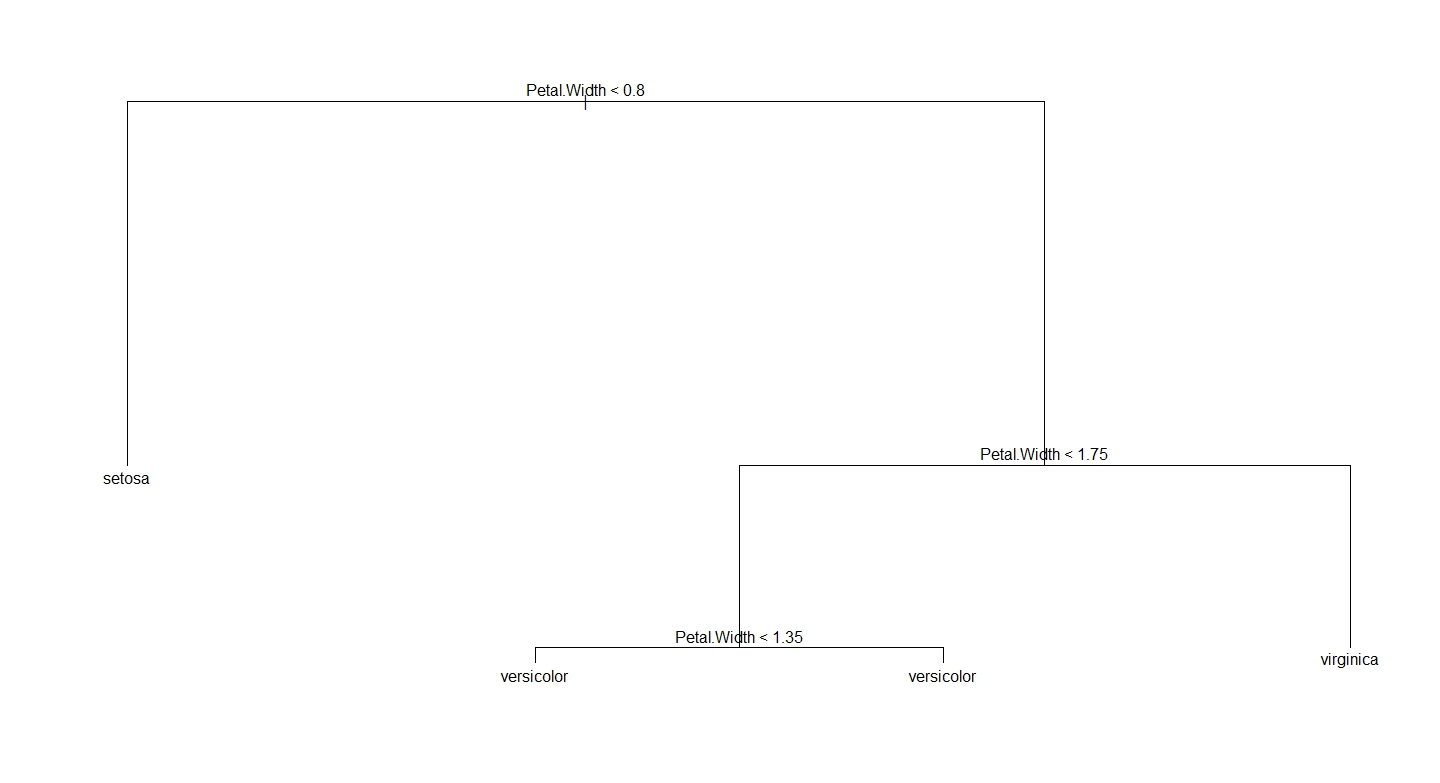
\includegraphics[width=0.99\linewidth]{./irispwtree}
\caption{}
\label{fig:irispwtree}
\end{figure}

\end{itemize}
\newpage
\subsection{Iris Tree Example}
\begin{itemize}
\item Using all four variables and all of the 150 cases
\end{itemize}

\begin{framed}
\begin{verbatim}
iris.tree <- tree(Species ~ Sepal.Length+Sepal.Width+
	Petal.Length+Petal.Width,data=iris)
plot(iris.tree)
text(iris.tree)

\end{verbatim}
\end{framed}

\begin{figure}[h!]
\centering
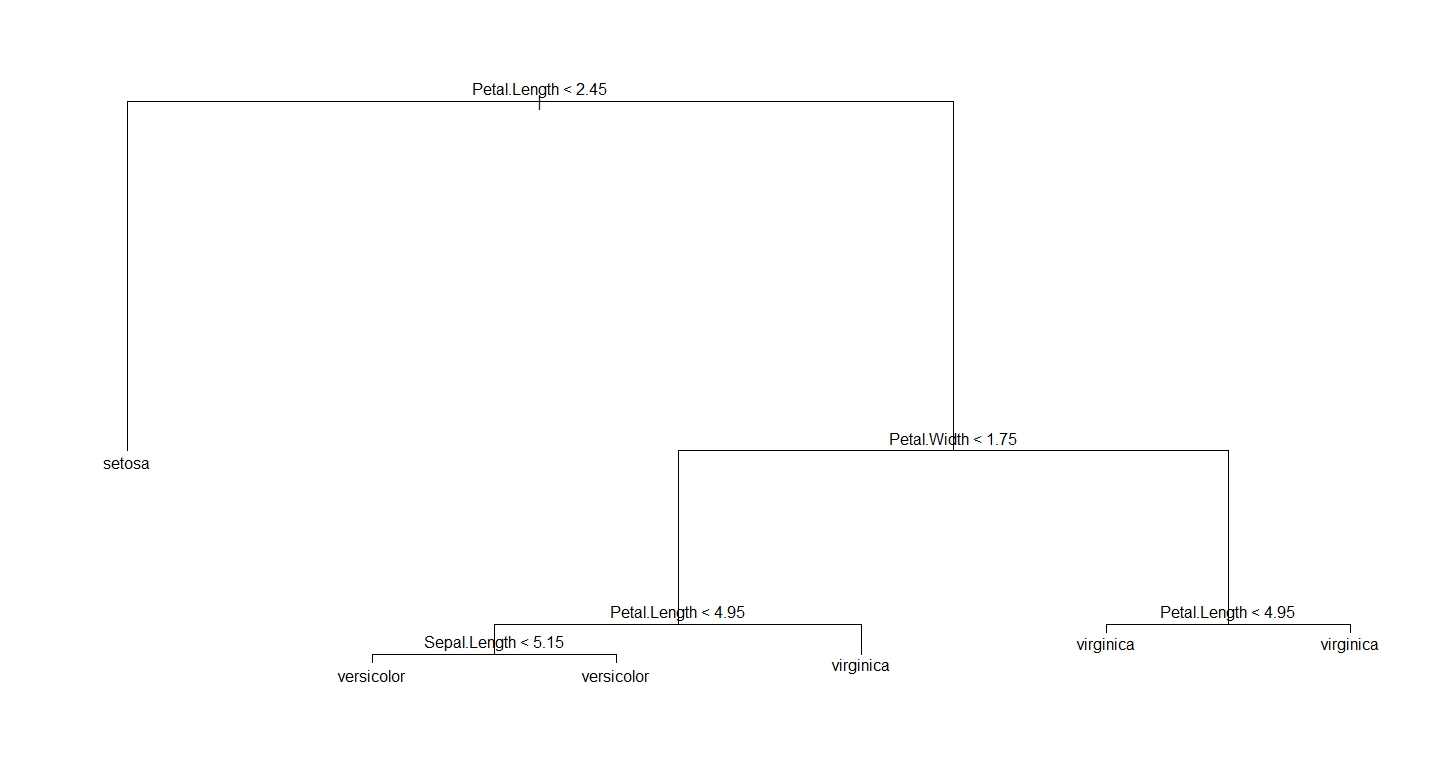
\includegraphics[width=0.8\linewidth]{./iristree1}
\caption{}
\label{fig:iristree1}
\end{figure}

\newpage
%-----------------------------------------------------------%
\subsubsection{Iris Example - Using a Training Set}
\begin{itemize}
\item set up a training data set of 100 randomly selected cases
\item Compare results with full data set tree.
\end{itemize}

\begin{framed}
\begin{verbatim}
set.seed(1234)
Train1Index = sample(1:150,100)
iristrain1=iris[Train1Index,]

iristrain1.tree <- tree(Species ~ Sepal.Length+Sepal.Width+
Petal.Length+Petal.Width,data=iristrain1)
plot(iristrain1.tree)
text(iristrain1.tree)
\end{verbatim}
\end{framed}
\begin{figure}[h!]
\centering
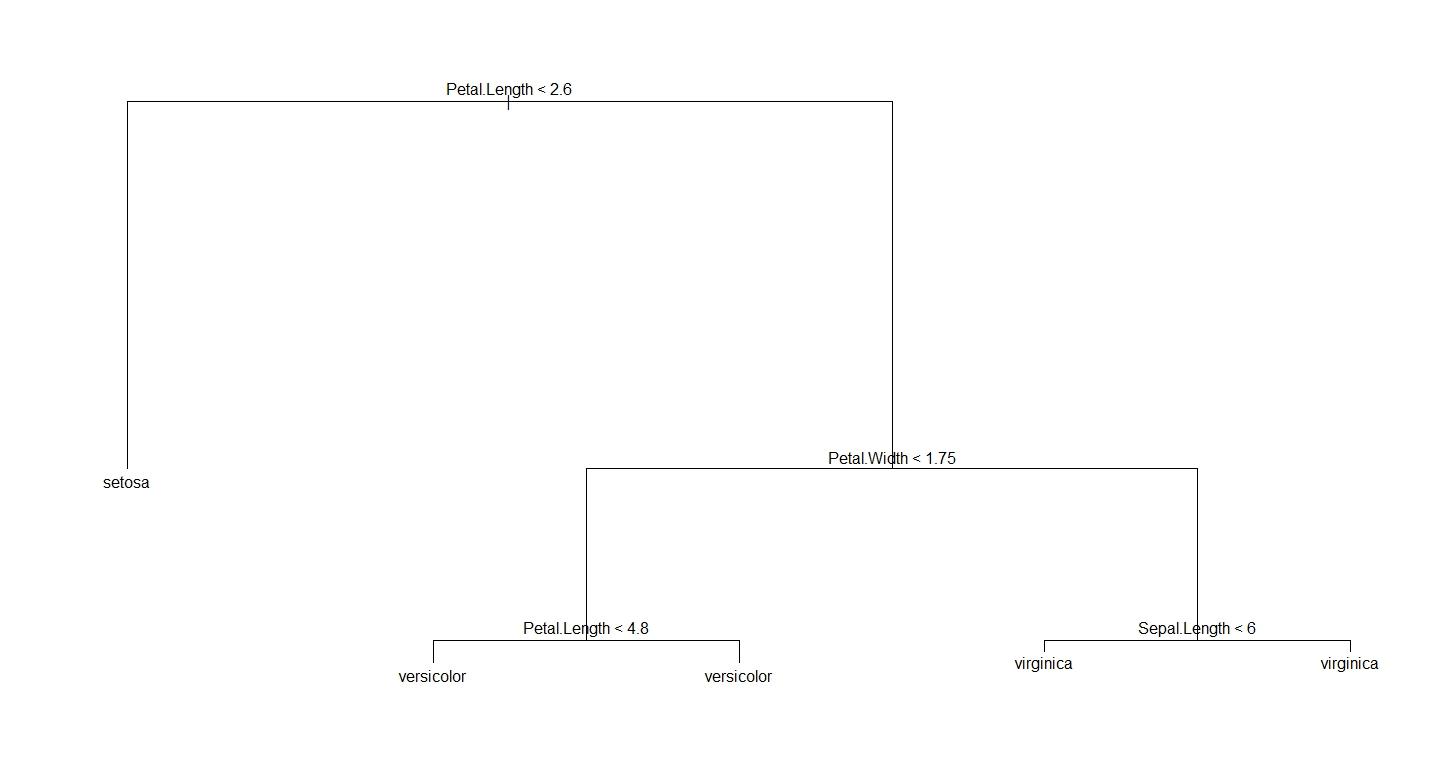
\includegraphics[width=0.80\linewidth]{./iristree2}
\caption{}
\label{fig:iristree2}
\end{figure}

\newpage
%-----------------------------------------------------------%

\begin{itemize}
\item Another test set (picked using a different seed)
\end{itemize}

\begin{framed}
\begin{verbatim}
set.seed(3456)

Train2Index = sample(1:150,100)
iristrain2=iris[Train2Index,]

iristrain2.tree <- tree(Species ~ Sepal.Length+Sepal.Width+
  Petal.Length+Petal.Width,data=iristtrain2)
plot(iristrain2.tree)
text(iristrain2.tree)
\end{verbatim}
\end{framed}
\begin{figure}[h!]
\centering
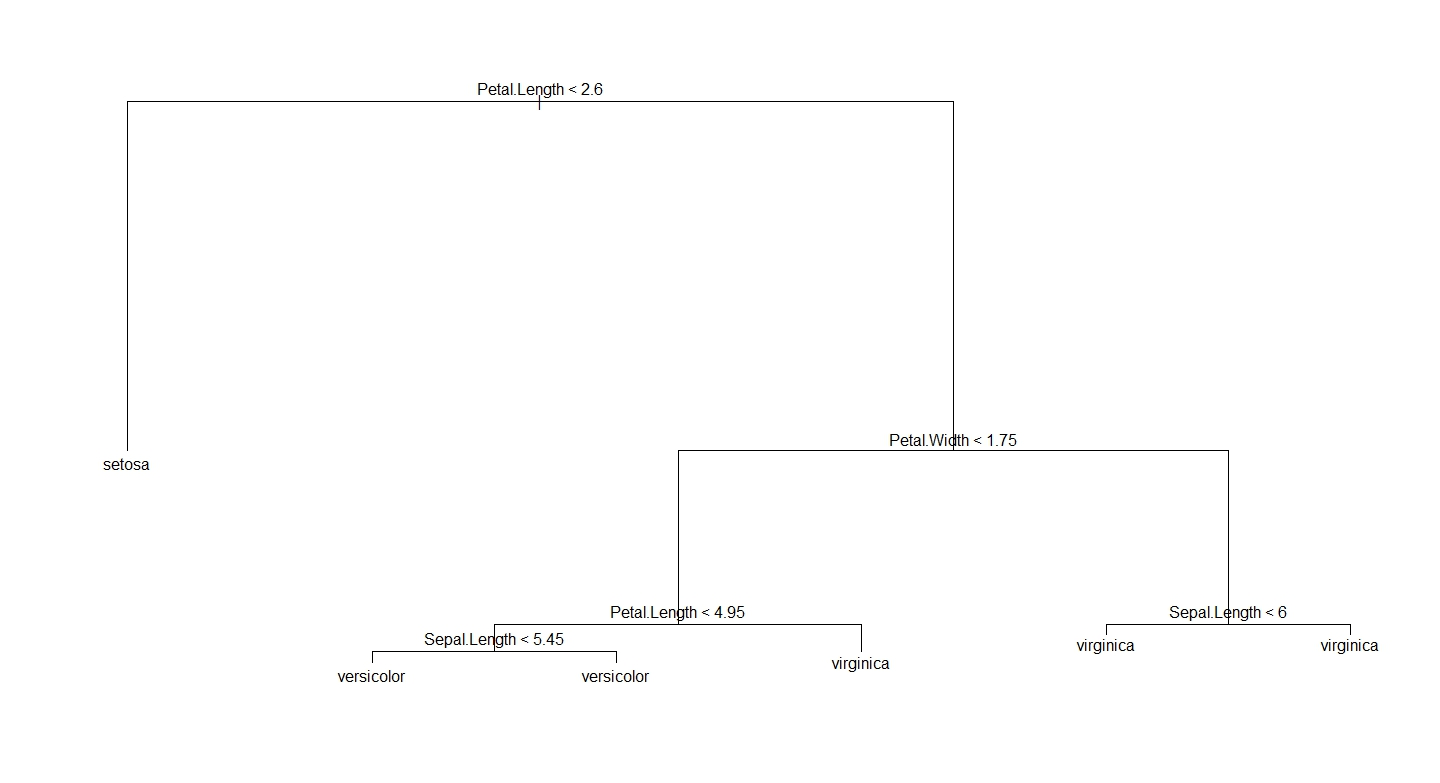
\includegraphics[width=0.80\linewidth]{./iristree3}
\caption{}
\label{fig:iristree2}
\end{figure}

\newpage
%-----------------------------------------------------------%


\begin{verbatim}
> table(iristrain1$Species)

    setosa versicolor  virginica 
        38         29         33 
> table(iristrain2$Species)

    setosa versicolor  virginica 
        34         32         34 
\end{verbatim}

\begin{itemize}
\item Set up a test data set to compare trees 
\item In this case, probably little difference
\end{itemize}

\begin{framed}
\begin{verbatim}
newdata=iris[131:150,]
predict(iristrain1.tree,newdata)
predict(iristrain2.tree,newdata)
\end{verbatim}
\end{framed}
\newpage
%------------------------------------------------------------------%
\subsection{Tree Pruning}
The \texttt{prune.tree()} command determines a nested sequence of subtrees
of the supplied tree by recursively snipping off the least important splits in
the classification tree.

\begin{framed}
\begin{verbatim}
iris.pruned <- prune.tree(iris.tree,best=3)
plot(iris.pruned); text(iris.pruned)
plot(iris.pruned); text(iris.pruned)
\end{verbatim}
\end{framed}
\begin{figure}[h!]
\centering
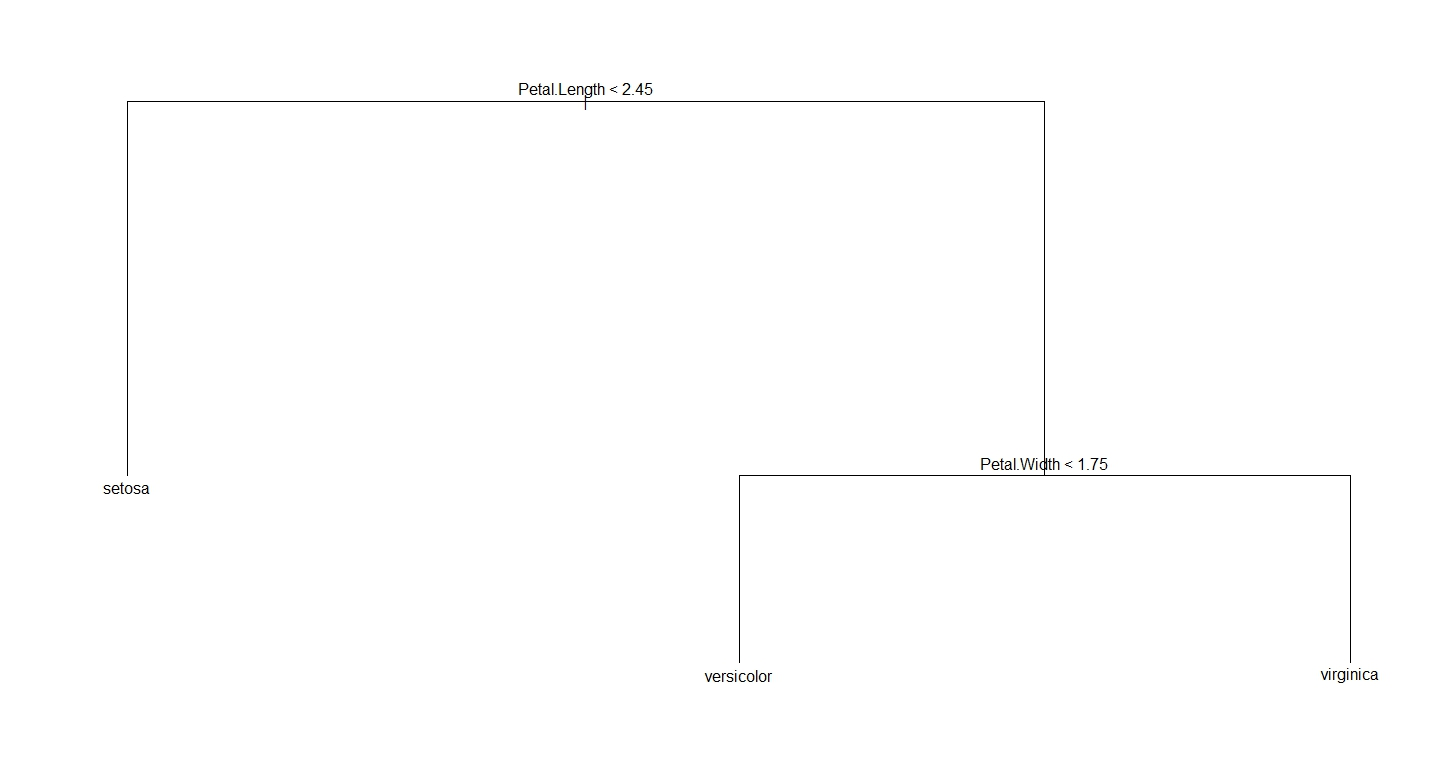
\includegraphics[width=0.9\linewidth]{./irispruned1}
\caption{}
\label{fig:irispruned1}
\end{figure}
\newpage
\subsection{Random Forests}
Random forests improve predictive accuracy by generating a large number of bootstrapped trees (based on random samples of variables), classifying a case using each tree in this new "forest", and deciding a final predicted outcome by combining the results across all of the trees (an average in regression, a majority vote in classification).



\begin{framed}
\begin{verbatim}
library(randomForest)
iris.rf <- randomForest(Species ~ Sepal.Length+Sepal.Width+
Petal.Length+Petal.Width,data=iris)
print(iris.rf) # view results 
importance(iris.rf) # importance of each predictor
\end{verbatim}
\end{framed}
\begin{verbatim}
> iris.rf <- randomForest(Species ~ Sepal.Length+Sepal.Width+
+ Petal.Length+Petal.Width,data=iris)
> print(iris.rf) # view results 

Call:
 randomForest(formula = Species ~ Sepal.Length + Sepal.Width +      Petal.Length + Petal.Width, data = iris) 
               Type of random forest: classification
                     Number of trees: 500
No. of variables tried at each split: 2

        OOB estimate of  error rate: 4%
Confusion matrix:
           setosa versicolor virginica class.error
setosa         50          0         0        0.00
versicolor      0         47         3        0.06
virginica       0          3        47        0.06
> importance(iris.rf) # importance of each predictor
             MeanDecreaseGini
Sepal.Length         9.654747
Sepal.Width          2.591063
Petal.Length        44.131695
Petal.Width         42.850817

\end{verbatim}
\subsection*{Making a Prediction}
\begin{framed}
\begin{verbatim}
library(randomForest)
iris.t1.rf <- randomForest(Species ~ Sepal.Length+Sepal.Width+
Petal.Length+Petal.Width,data=iristest1)


newdata2index=sample(1:150,20)
newdata2=iris[newdata2index,]

predict(iris.t1.rf,newdata2)
\end{verbatim}
\end{framed}
\newpage
\subsection{Regression Trees}

\begin{itemize}
\item The general approach to derive predictions from few simple \texttt{if-then} conditions can be applied to regression problems as well. 
\item In this example, we will use the \texttt{cu.summary} data set in the \textbf{\textit{rpart}} package.
\end{itemize}

\begin{verbatim}
> library(rpart)
> tail(cu.summary)
                     Price Country Reliability Mileage Type
Ford Aerostar V6     12267     USA     average      18  Van
Mazda MPV V6         14944   Japan Much better      19  Van
Mitsubishi Wagon 4   14929   Japan        <NA>      20  Van
Nissan Axxess 4      13949   Japan        <NA>      20  Van
Nissan Van 4         14799   Japan        <NA>      19  Van
Volkswagen Vanagon 4 14080 Germany        <NA>      NA  Van
\end{verbatim}



\begin{framed}
\begin{verbatim}
fit <- rpart(Mileage~Price + Country + Reliability + Type, 
   method="anova", data=cu.summary)

printcp(fit) # display the results 
\end{verbatim}
\end{framed}
\newpage
\subsection*{Display results of fitted tree}

\begin{verbatim}
> printcp(fit) # display the results 

Regression tree:
rpart(formula = Mileage ~ Price + Country + Reliability + Type, 
    data = cu.summary, method = "anova")

Variables actually used in tree construction:
[1] Price Type 

Root node error: 1354.6/60 = 22.576

n=60 (57 observations deleted due to missingness)

        CP nsplit rel error  xerror     xstd
1 0.622885      0   1.00000 1.00671 0.174008
2 0.132061      1   0.37711 0.52578 0.099645
3 0.025441      2   0.24505 0.36496 0.077946
4 0.011604      3   0.21961 0.35238 0.078224
5 0.010000      4   0.20801 0.35522 0.074295

\end{verbatim}
\newpage
\begin{framed}
\begin{verbatim}
# plot the regression tree 
plot(fit, uniform=TRUE, 
  	main="Regression Tree for Mileage ")
text(fit, use.n=TRUE, all=TRUE, cex=1.0)

\end{verbatim}
\end{framed}

\begin{figure}[h!]
\centering
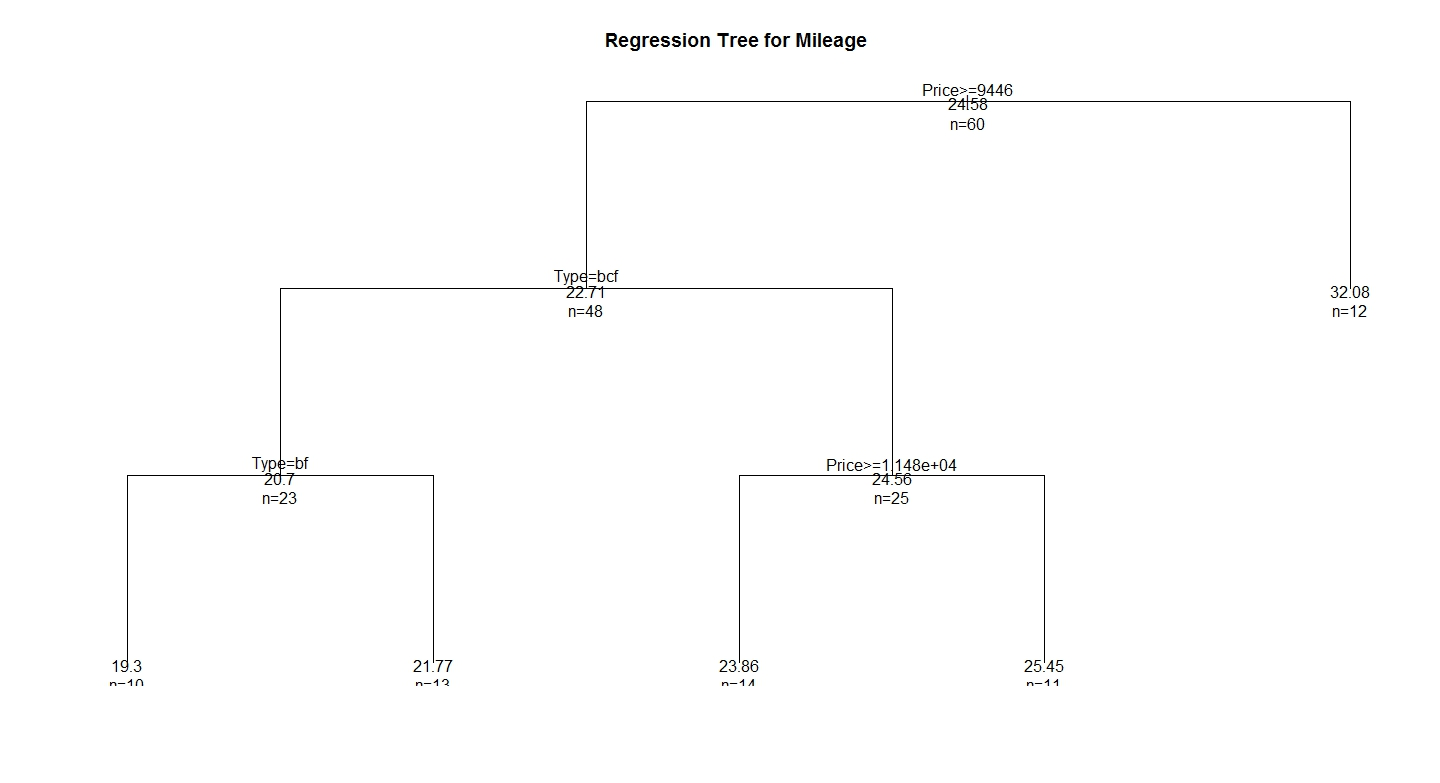
\includegraphics[width=0.99\linewidth]{./regresstree1}
\caption{}
\label{fig:regresstree1}
\end{figure}
\newpage
Compare predicted values with observed values.
\begin{verbatim}
> cbind(predict(fit,cu.summary),cu.summary$Mileage)
                                  [,1] [,2]
Acura Integra 4               23.85714   NA
Dodge Colt 4                  32.08333   NA
Dodge Omni 4                  32.08333   NA
Eagle Summit 4                32.08333   33
Ford Escort   4               32.08333   33
Ford Festiva 4                32.08333   37
GEO Metro  3                  32.08333   NA
GEO Prizm  4                  25.45455   NA
................
\end{verbatim}
%---------------------------------------------------------------------------------------%
\newpage
\subsection{Advantages of Classification and Regression Trees (CaRT) Methods}

\begin{itemize}
\item As mentioned earlier, there are a large number of methods that an analyst can choose from when analyzing classification or regression problems. 
\item Tree classification techniques, when they "work" and produce accurate predictions or predicted classifications based on few logical if-then conditions, have a number of advantages over many of those alternative techniques.

\item \textbf{Simplicity of results} - In most cases, the interpretation of results summarized in a tree is very simple. This simplicity is useful not only for purposes of rapid classification of new observations (it is much easier to evaluate just one or two logical conditions, than to compute classification scores for each possible group, or predicted values, based on all predictors and using possibly some complex nonlinear model equations), but can also often yield a much simpler "model" for explaining why observations are classified or predicted in a particular manner (e.g., when analyzing business problems, it is much easier to present a few simple \textit{if-then} statements to management, than some elaborate equations).

\item Tree methods are nonparametric and nonlinear. The final results of using tree methods for classification or regression can be summarized in a series of (usually few) logical if-then conditions (tree nodes). Therefore, there is no implicit assumption about underlying relationships between between variables.
 
\item Thus, tree methods are particularly well suited for data mining tasks, where there is often little a priori knowledge nor any coherent set of theories or predictions regarding which variables are related and how. In those types of data analyses, tree methods can often reveal simple relationships between just a few variables that could have easily gone unnoticed using other analytic techniques.
\end{itemize}
\newpage

%------------------------------------------------------------------------%
%\subsection{General Computation Issues and Unique Solutions of CaRT}

%The computational details involved in determining the best split conditions to construct a simple yet useful and informative tree are quite complex. 
%Refer to Breiman et al. (1984) for a discussion of their CART® algorithm to learn more about the general theory of and specific computational solutions for constructing classification and regression trees.
% An excellent general discussion of tree classification and regression methods, and comparisons with other approaches to pattern recognition and neural networks, is provided in Ripley (1996).

% Resampling
\subsection{Avoiding Over-Fitting: Pruning, Crossvalidation, and V-fold Crossvalidation}
\begin{itemize}
\item A major issue that arises when applying regression or classification trees to "real" data with much random error noise concerns the decision when to stop splitting. For example, if we had a data set with 20 cases, and performed 19 splits (determined 9 if-then conditions), we could perfectly predict every single case. 
\item In general, if we only split a sufficient number of times, eventually we will be able to "predict" our original data (from which we determined the splits). Of course, it is far from clear whether such complex results (with many splits) will replicate in a sample of new observations; most likely they will not.

\item \textbf{Overfitting} -
This general issue is relevant to tree classification (as well as neural networks and regression methods)
\item  If not stopped, the tree algorithm will ultimately "extract" all information from the data, including information that is not and cannot be predicted in the population with the current set of predictors, i.e., random or noise variation.
\item The general approach to addressing this issue is first to stop generating new split nodes when subsequent splits only result in very little overall improvement of the prediction.
\item For example, if we can predict 90\% of all cases correctly from 10 splits, and 90.1\% of all cases from 11 splits, then it obviously makes little sense to add that 11th split to the tree.

\end{itemize}
\subsubsection*{Criteria}
There are many such criteria for automatically stopping the splitting (tree-building) process.
\begin{itemize}
\item \textbf{Pruning} - Once the tree building algorithm has stopped, it is always useful to further evaluate the quality of the prediction of the current tree in samples of observations that did not participate in the original computations. These methods are used to "prune back" the tree, i.e., to eventually (and ideally) select a simpler tree than the one obtained when the tree building algorithm stopped, but one that is equally as accurate for predicting or classifying "new" observations.
\item
\textbf{Cross-validation} -  One approach is to apply the tree computed from one set of observations (training sample) to another completely independent set of observations (testing sample). If most or all of the splits determined by the analysis of the training sample are essentially based on "random noise," then the prediction for the testing sample will be very poor. Hence, we can see if the selected tree is not very good (useful), or not of the "right size."

\item \textbf{V-fold crossvalidation} Continuing further along this line of reasoning, we repeat the analysis many times over with different randomly drawn samples from the data, for every tree size starting at the root of the tree, and applying it to the prediction of observations from randomly selected testing samples. 
\item Then use the tree that shows the best average accuracy for cross-validated predicted classifications or predicted values.
\item In most cases, this tree will not be the one with the most terminal nodes, i.e., the most complex tree. This method for pruning a tree, and for selecting a smaller tree from a sequence of trees, can be very powerful, and is particularly useful for smaller data sets. 
\end{itemize}
\newpage


\subsection{Computational Details}

The process of computing classification and regression trees can be characterized as involving four basic steps:

\begin{enumerate}
\item Specifying the criteria for predictive accuracy
\item Selecting splits
\item Determining when to stop splitting
\item Selecting the "right-sized" tree.
\end{enumerate}
%These steps are very similar to those discussed in the context of Classification Trees Analysis (see also Breiman et al., 1984, for more details).
% See also, Computational Formulas.

\newpage 


\begin{framed}
\begin{verbatim}

library(caret)
set.seed(3456)

#Split the data in training and testing data

trainIndex <- createDataPartition(iris$Species, p = .8,
                                  list = FALSE,
                                  times = 1)
head(trainIndex)

irisTrain <- iris[ trainIndex,]
irisTest  <- iris[-trainIndex,]

# Fit a model using the training data
iris.caret <- train(Species ~ ., data = irisTrain,
   method = "rpart", maxdepth=4)

iris.caret

# Try it out on the testing data
iris.caret.test <- predict(iris.caret,irisTest)


table(iris.caret.test,irisTest$Species)

\end{verbatim}
\end{framed}
\begin{verbatim}
> table(iris.caret.test,irisTest$Species)
               
iris.caret.test setosa versicolor virginica
     setosa         10          0         0
     versicolor      0         10         0
     virginica       0          0        10

\end{verbatim}



\subsection{Specifying the Criteria for Predictive Accuracy}

The classification and regression trees (C\&RT) algorithms are generally aimed at achieving the best possible predictive accuracy. Operationally, the most accurate prediction is defined as the prediction with the minimum costs. The notion of costs was developed as a way to generalize, to a broader range of prediction situations, the idea that the best prediction has the lowest misclassification rate. In most applications, the cost is measured in terms of proportion of misclassified cases, or variance. In this context, it follows, therefore, that a prediction would be considered best if it has the lowest misclassification rate or the smallest variance. The need for minimizing costs, rather than just the proportion of misclassified cases, arises when some predictions that fail are more catastrophic than others, or when some predictions that fail occur more frequently than others.

\end{document}